\chapter{Validation des méthodes numériques}

On s'intéresse d'abord à des cas de référence dans lesquels tous les carreaux ont un domaine paramétrique égal à $\chebinterval \times \chebinterval$, ce qui permet d'effectuer des mesures de précisions à la fois locales (position de l'interface) et globales (aire et volume délimité, par quadrature). 
Pour cela, on choisit des géométries simples et sans arête concave.
(On pourrait étendre les formules de quadrature aux carreaux restreints, voir IGA.)

\section{Propagation suivant un champ de vitesse analytique}

sphère dans un écoulement tourbillonnaire incompressible analytique de période temporelle $2T$
\begin{equation}
	\vrm{u}(x,y,z,t) = 
	%\cos \left( \frac{\pi t}{T} \right)
	\cos( \pi t/T )
	\colvec{
	\sin^2(\pi x) \left[ \sin(2\pi z) - \sin(2\pi y)\right] \\
\sin^2(\pi y) \left[ \sin(2\pi x) - \sin(2\pi z)\right] \\
\sin^2(\pi z) \left[ \sin(2\pi y) - \sin(2\pi x)\right]
	}.
\end{equation}

\begin{figure}
	\centering
	\setlength{\imagewidth}{0.49\linewidth}%
\newdimen\imypos
\imypos=1.1\imagewidth
\begin{tikzpicture}[%
	img/.style={anchor=north west, inner sep=0},%
	txt/.style={font=\normalsize, inner sep=2pt, anchor=south west}%
	]%
	%
	\begin{scope}%
	\clip(0,-0.15\imagewidth) rectangle (2\imagewidth, -2\imagewidth);
	\node[img] (im1) at (          0,         0) {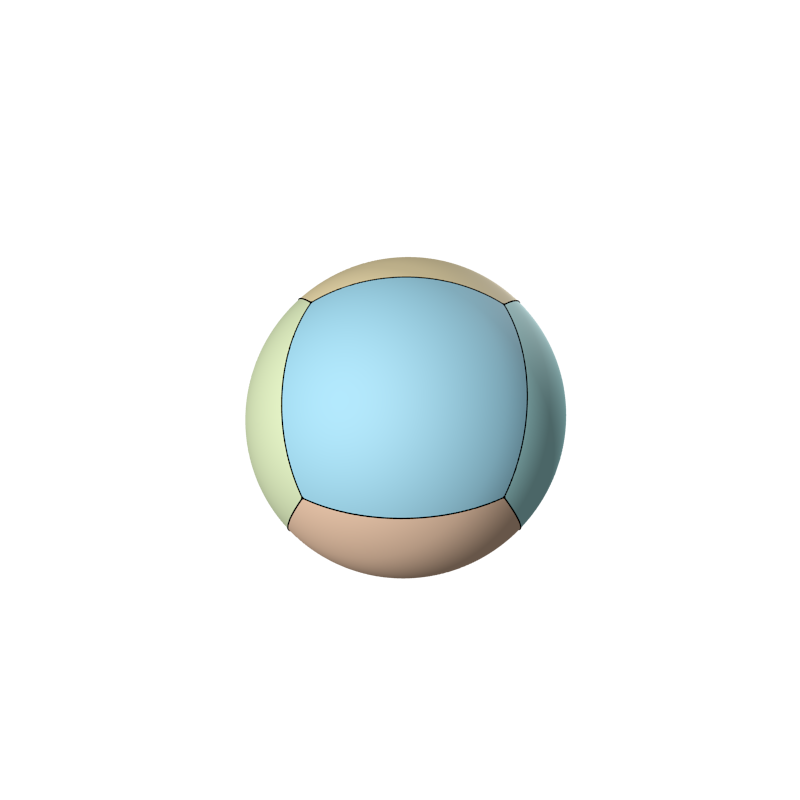
\includegraphics[width=\imagewidth]{vortex/snap_001}};
	\node[img] (im2) at (\imagewidth,         0) {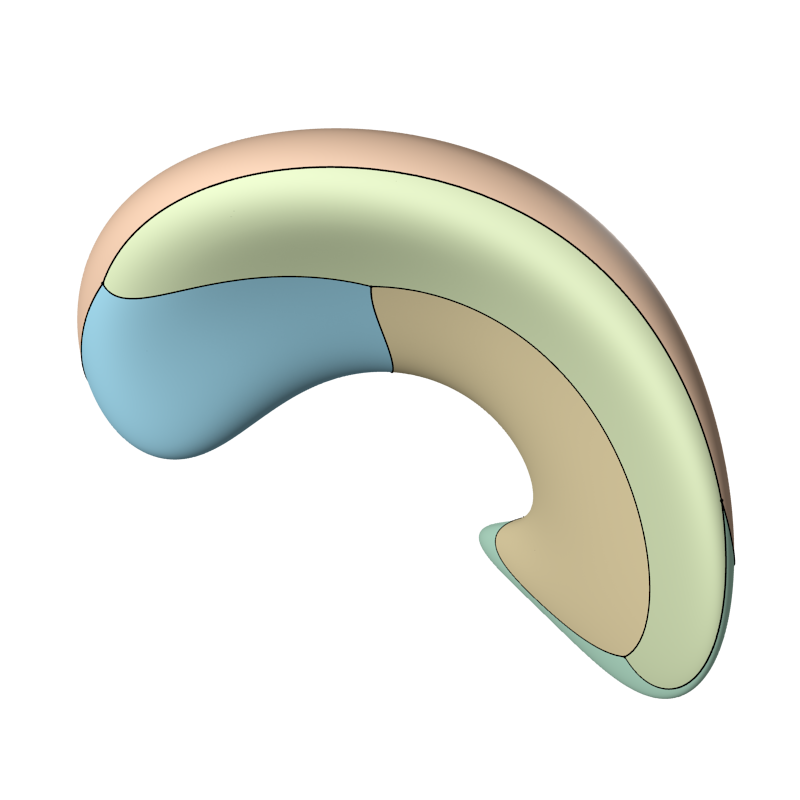
\includegraphics[width=\imagewidth]{vortex/snap_002}};
	\end{scope}%
	\node[img] (im3) at (          0,  -\imypos) {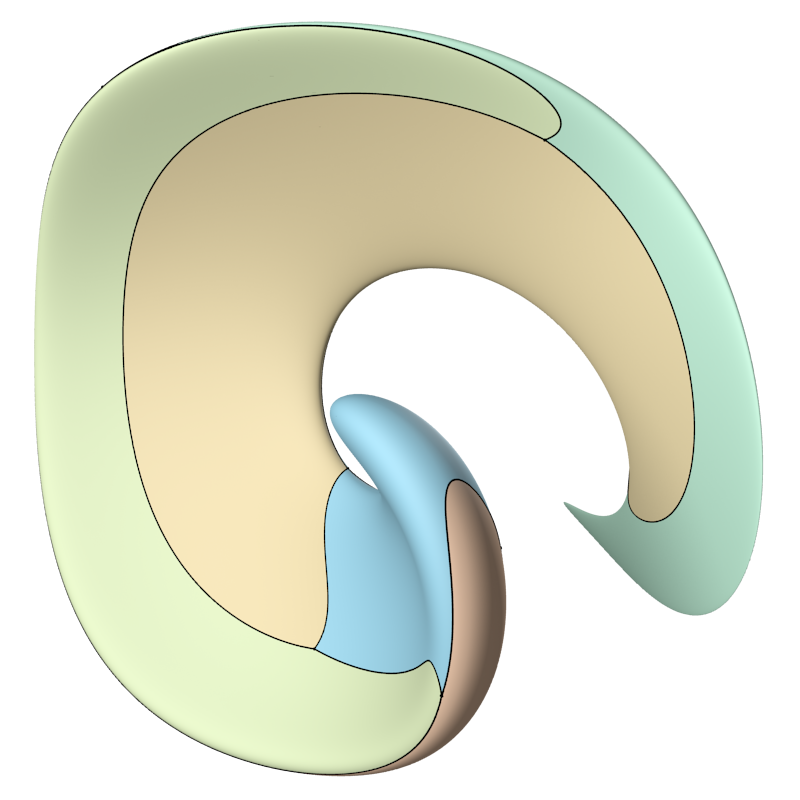
\includegraphics[width=\imagewidth]{vortex/snap_003}};
	\node[img] (im4) at (\imagewidth,  -\imypos) {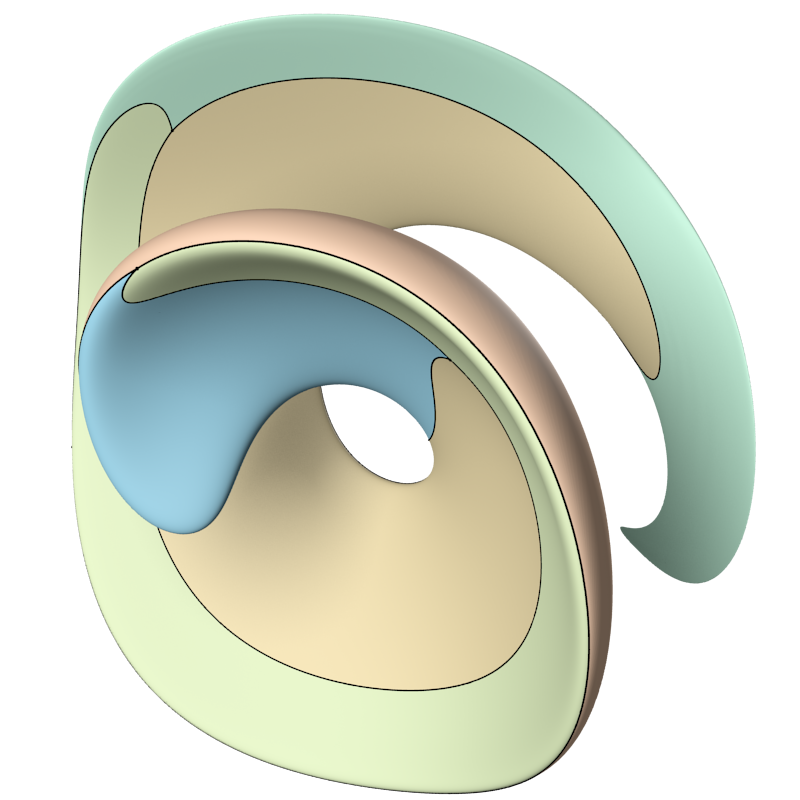
\includegraphics[width=\imagewidth]{vortex/snap_004}};
	\node[img] (im5) at (          0, -2\imypos) {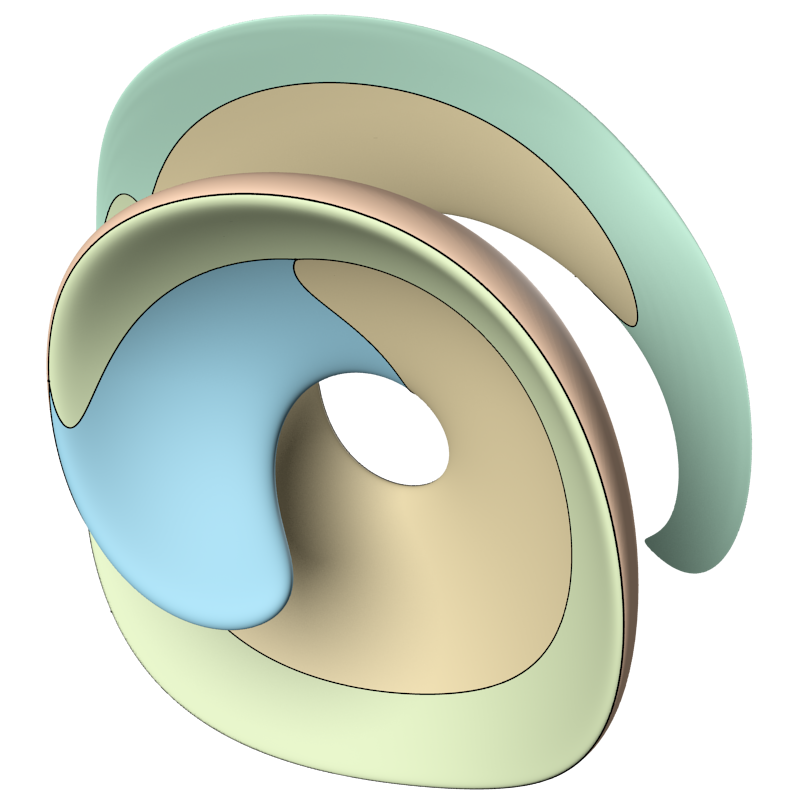
\includegraphics[width=\imagewidth]{vortex/snap_005}};
	\node[img] (im6) at (\imagewidth, -2\imypos) {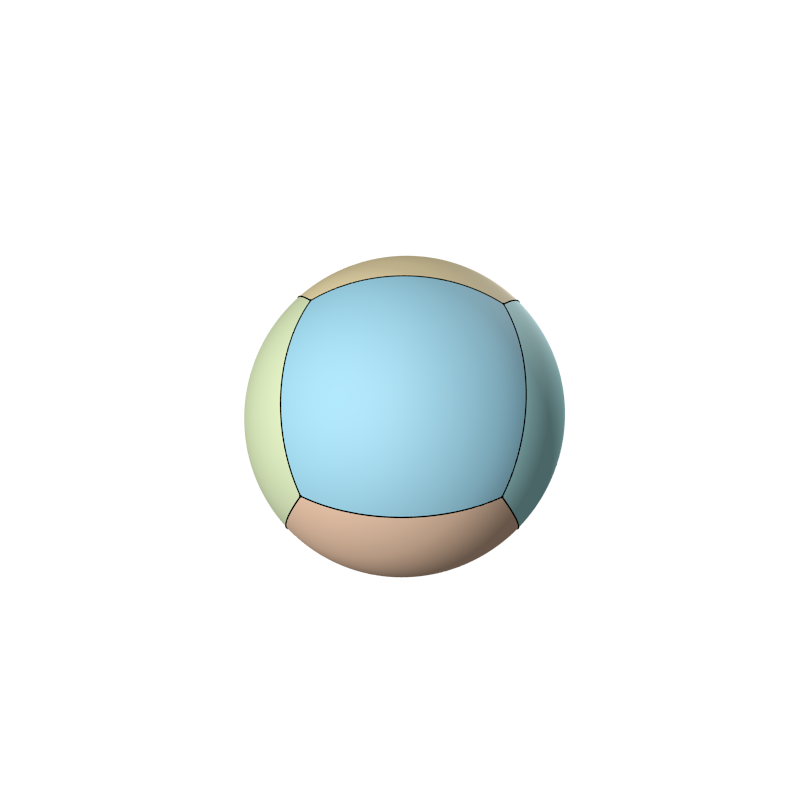
\includegraphics[width=\imagewidth]{vortex/snap_006}};
	%
	\node[txt] at (im1.south west) {$t=   0$};
    \node[txt] at (im2.south west) {$t= T/8$};
    \node[txt] at (im3.south west) {$t= T/4$};
    \node[txt] at (im4.south west) {$t=3T/8$};
    \node[txt] at (im5.south west) {$t= T/2$};
    \node[txt] at (im6.south west) {$t=   T$};
\end{tikzpicture}
	\caption{Aperçu du modèle \brep\ de la sphère dans un écoulement tourbillonnaire à différents instants de la propagation ($T=4$).}
	\label{fig:snapshots_vortex}
\end{figure}

\begin{enumerate}
	\item paramétrisation initiale : grille CGL des faces d'un cube projetées sur la sphère% ou \guillemets{slerp}
	\item calcul de l'aire : intégration (approchée) par quadrature de Clenshaw-Curtis de l'élément d'aire $\sqrt{\determinant{\fff}}$
	\item calcul de volume : formule de Green avec quadrature exacte car l'intégrande est polynomiale %(étanchéité (continuité $\contgeom{0}$ partout) garantie car les marqueurs de bord coïncident tout au long de la déformation)
	\item critère d'erreur sur la position : distance à la sphère exacte
	\item convergence de l'erreur d'approximation sur la position (\autoref{fig:vortex_error_vs_dof_pos}), l'aire (\autoref{fig:vortex_error_vs_dof_air}) et le volume (\autoref{fig:vortex_error_vs_dof_vol}) à $t = 0$ et $t = T$ pour différents niveaux de discrétisations spatiale et temporelle 
	\begin{itemize}
		\item[$\to$] l'approximation de la sphère initiale converge rapidement avec le degré du polynôme d'interpolation(\ie le nombre de degrés de liberté)
		\item[$\to$] si la résolution spatiale est suffisamment fine, l'erreur d'approximation est essentiellement due à la discrétisation temporelle
	\end{itemize}
	\item convergence de la variation de volume au cours de la déformation (censée être nulle car $\nabla \cdot \vrm{u} = 0$) (\autoref{fig:vortex_error_volume_vs_time})
	\begin{itemize}
		\item[$\to$] on retrouve une convergence rapide : le pic à $t = T/2$ décroît exponentiellement avec $N$ 
	\end{itemize}
\end{enumerate}

%\\
%calcul de volume avec quadrature de Clenshaw-Curtis (exact, l'intégrande est polynomiale) (étanchéité (continuité $\contgeom{0}$ partout) garantie car les marqueurs de bord coïncident tout au long de la déformation)\\
%convergence de l'erreur d'approximation sur la position, l'aire et le volume à $t = 0$ et $t = T$ pour différents niveaux de discrétisations spatiale et temporelle\\

%%%%%%%%%%%%%%%%%%%%%%%%%%%%%
% FIGURES ERREUR VS DOF
\def\axw{0.48\textwidth}
\def\axh{0.39\textwidth}
\def\xlabl{$N$}%{$\mathrm{dof}$}
\def\ylabl{Erreur}
\def\xsep{2pt}
%%% POSITION
\plotVortexErrorVsDof{position}{la~}{pos}{maximale}
%%% AIRE
\plotVortexErrorVsDof{aire}{l'}{air}{relative}
%%% VOLUME
\plotVortexErrorVsDof{volume}{le~}{vol}{relative}
%%%%%%%%%%%%%%%%%%%%%%%%%%%%

%+ convergence de la variation de volume au cours de la déformation (censée être nulle)\\
\begin{figure}
  \centering
  \begin{tikzpicture}%
  \begin{semilogyaxis}[%
    axis lines*=left,%
    width=9cm, height=7cm,%
    xmin = 0.0, xmax = 1.0,%
    ymin = 1e-16, ymax = 1e0,%
    ytickten = {-16,-12,-8,-4,0},%
    xtick distance=.25,
    grid=major,%
    xlabel={$t/T$},%
    ylabel={$\frac{\left|V - V_0\right|}{V_0}$},%
    legend style={font=\small, at={(0.5,0.033)}, anchor=south},%
    no marks, each nth point=1]%
    \pgfplotstableread{figures/data/vortex/vortex_erreur_volume_vs_time_0.001.dat}{\datatable}
    \pgfplotstablegetcolsof{\datatable}
    \pgfmathtruncatemacro\numberofcols{\pgfplotsretval-1}
    \pgfplotsinvokeforeach{1,...,\numberofcols}{%
		\pgfplotstablegetcolumnnamebyindex{#1}\of{\datatable}\to{\colname}%
		\addplot+ table [y index=#1] from \datatable;% node[right, pos=1, anchor=west] {$N = \colname$};%
		\addlegendentryexpanded{$N = \colname$}%
    }%
  \end{semilogyaxis}%
  \end{tikzpicture}%
  \caption{Évolution au cours du temps de l'erreur relative en volume pour différents niveaux de discrétisation spatiale. Le schéma de Runge-Kutta explicite à l'ordre 4 est utilisé pour l'intégration temporelle, avec un pas de temps $\Delta t = 0.001$.}
  \label{fig:vortex_error_volume_vs_time}
\end{figure}

Nuancer la pertinence de ce cas test :
\begin{itemize}
	\item pour d'autres cas test analogues (\eg cas test de Enright), un mouvement tangentiel (reparamétrisation) des marqueurs lagrangiens est nécessaire pour garantir la stabilité numérique
	\item mais ce type de déformation extrême n'est pas celui que l'on vise dans nos applications, ce pourquoi on n'a pas plus considéré la reparamétrisation
	\item permet toutefois d'évaluer le pouvoir de résolution des polynômes de Chebyshev et vérifier la convergence rapide de l'erreur dapproximation
\end{itemize}

\section{Propagation à vitesse normale uniforme}
cube en expansion à vitesse normale uniforme $\nu = 1$

\begin{figure}
	\centering
	\newdimen\imwid
	\imwid=0.32\linewidth
	\begin{tikzpicture}
		\foreach [count=\i] \l in {{0}, {1}, {2}}
		{%
			\node (im\i) at (\i\imwid,0) {\includegraphics[width=\imwid]{expanding_cube/cube_brep_t\i}};
			\node[inner sep=0pt] (lab\i) at (im\i.south) {$t = \l$};
		}%
	\end{tikzpicture}
	\caption{Aperçu du modèle \brep\ du cube en expansion à différents instants de la propagation.}
	\label{fig:snapshots_cube}
\end{figure}

\begin{enumerate}
	\item stratégie pour la pseudo-EdS des sommets : polygone découpé en quads (\cf \autoref{section:quadrangulation_polygone_spherique}) pour évaluer simplement l'aire et le volume par quadrature (possible car $\nu$ est uniforme)
	\item critère d'erreur sur la position : erreur relative sur la distance au cube (car la solution exacte est une iso-surface de la fonction distance)
	\item convergence de l'erreur d'approximation sur la position, l'aire et le volume à $t = 2$ pour différents niveaux de discrétisations spatiale et temporelle (voir \autoref{fig:convergence_cube})
\end{enumerate}



\begin{figure}
	\centering
	\begin{tikzpicture}[inner frame sep=0]%
      \begin{semilogyaxis}[%
      %scale only axis,%
      axis lines*=left,%
      width=8cm, height=6cm,%
      xmin = 0, xmax = 20,% 
      ymin = 1e-16, ymax = 1,%
      xtick={0,5,10,15,20},%
      ytickten = {-16,-12,-8,-4,0},%
      grid=major,%both,%
      xlabel={$N$},%_{\mathrm{max}}$}, 
      ylabel={Erreur},%\ylabl},%
      legend style={font=\small},%
      legend pos=north east,%south west,%
      cycle list shift=0]%
	  \pgfplotstableread{figures/data/convergence_expanding_cube.dat}  {\datatable}%
	  \pgfplotstablegetcolsof{\datatable}%
      \pgfmathtruncatemacro\numberofcols{\pgfplotsretval-1}%
      \pgfplotsinvokeforeach{3,...,\numberofcols}{%
        \pgfplotstablegetcolumnnamebyindex{#1}\of{\datatable}\to{\colname}%
        %https://tex.stackexchange.com/questions/317225/automatic-labelling-of-isolines-based-on-tables-column-name
		\addplot table [x index=0, y index=#1] from \datatable;
  	    \addlegendentryexpanded{\colname}%
      }%
      \end{semilogyaxis}%
    \end{tikzpicture}%
	\caption{Erreurs sur la position l'aire et le volume pour différents niveaux de discrétisations spatiale et temporelle, à $t = 2$.}
	\label{fig:convergence_cube}
\end{figure}

Intérêts de ce cas test :
\begin{itemize}
	\item valider l'approximation du vecteur normal unitaire 
	\item valider la construction des pseudo-EdS des arêtes et sommets \brep\ convexes
\end{itemize}


\par\bigskip
\textit{
	[Bilan du chapitre et transition vers le chapitre suivant\ldots]
}
